%This is chapter 2
%%=========================================
\chapter{Theoretical basis}

%%=========================================
\section{Agile methods}
\subsection{Scrum}
Scrum is an agile methodology. 
Background and history of the evolution of scrum......
What is it? How does it work?

\subsection{Kanban}

\section{Git}
Git is a type of distributed version control system (VCS), originally created by Linus Torvalds in 2005. Git is free and opensource, and is today the most popularly used VCS. It is fast and efficient, able to handle everything from small hobby projects to giant projects like the Linux kernel. Every Git directory is a complete repository with history and full version-tracking abilities. It does not need access to internet, nor a central server in order to work.

\subsection{GitFlow}
GitFlow is a popular branching model for Git, created by \cite{gitflow}. Figure \ref{fig:gitflow} displays an example git history, adhering the GitFlow branching style.
\begin{figure}[h]
    \centering
    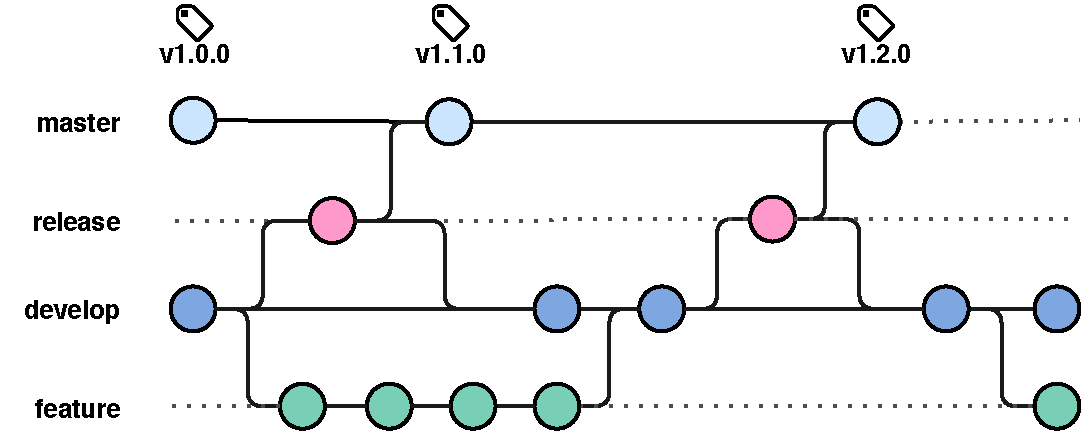
\includegraphics[page=1,width=\textwidth]{sections/methodology/figures/gitflow.pdf}
    \caption{GitFlow branching model example.}
    \label{fig:gitflow}
\end{figure}

\section{GitHub}
GitHub is primarily a hosting service for Git repositories. The company was acquired by Microsoft in 2019. In addition to repository hosting, GitHub provides a range of different services through it's web-based GUI. This includes both wikis, access controls, simple task management tools, automation capabilities and websites hosting.

\subsection{GitHub Actions}
GitHub Actions \cite{github-actions} is a fairly very new service provided by GitHub. It enables users to automate software workflows, effectively providing a high quality CI/CD for free \footnote{GitHub Actions usage is completely free for public repositories. For private repositories, depending on the subscription plan, some thousand minutes of free usage is provided each month.}. It is also possible to set up self-hosted runners. GitHub Actions makes it possible to both build, test and deploy code directly from within GitHub.

\subsection{GitHub Pages}
Github provides its users with a public webpage hosting service. This is named GitHub Pages \cite{github-pages}. User are able to serve static websites directly from their repository hosted on GitHub.

\section{HyperText Markup Language (HTML)}
HTML is a markup language, originally defined by Tim Berners-Lee and Robert Caillau in 1989. It is primarily used for documents on the web, intended to be displayed in a web-browser. It is used for structuring and formatting information. HTML can be used in conjunction with other web technologies such as Cascading Style Sheets (CSS) and scripting languages like JavaScript, in order to either style or dynamically change and alter the contents of a web page. The currently latest release of the language is HTML5.

\section{Cascading Style Sheets (CSS)}
CSS is short for Cascading Style Sheets. CSS is a programming language in order to describe how HTML elements in a HTML file are to be rendered. Everything from the boldness of a headline, to the background of the entire page.

\section{JavaScript}
JavaScript is a lightweight interpreted programming language. The language is prototype-based, a type of object-oriented programming where properties and methods are added to an instance of an implicitly defined class \cite{prototype-based-programming}.

JavaScript was developed by Brendan Eichand and released in 1995 \cite{javascript-original-release}. Initially, it was designed to be a small scripting language for enabling interaction with web pages. A standardization effort of JavaScript, led by Ecma International \cite{ecma-international}, lead to the ECMAScript specification.  that the modern JavaScript language conforms to. Several releases. Since then, the language has evolved rapidly and gained massive in popularity. It has become the de-facto language for adding dynamic behavior to HTML. As of may 2020, JavaScript is among the top ten programming languages according to the TIOBE index \cite{tiobe-index}.

% Node.js
Originally, JavaScript engines were mainly used in browser environments. However, with the development of Node.js in early 2009, this was dramatically changed. Node.js provides a runtime environment for executing JavaScript outside of a web browser. It set the stage for server-side JavaScript programs. In January 2010, a package manager named npm \cite{npm} was released for Node.js. This made it easy for developers to share and use source code.

% Module bundlers
The size of JavaScript programs has increased massively in size. With increased size, so does the complexity of the code. However, JavaScript had very limited functionality in terms of splitting a program up in smaller modules for use with the browser. Maintaining large codebases was a nightmare. It therefore became apparent that a way of breaking down a JavaScript program into smaller modules was needed. Several open-source module systems were therefore developed by the community in order to tackle this problem.

\subsection{Module systems}
\begin{itemize}
    \item \textbf{CommonJS} is a module specification meant for JavaScript outside the browser. It is mainly used in Node.js, and hence it is one of the most popularly used module definitions. The modules are mainly imported and exported with the keywords "require" and "module.exports".
    \item \textbf{Asynchronous module definition}, or more commonly known as AMD, is a JavaScript module definition intended for the browser. It defines an API for defining code as modules, including their dependencies. AMD also has the capability of loading modules asynchronously. The most popular AMD module loader is named RequireJS \cite{requirejs}.
    \item \textbf{Universal Module Definition}, abbreviated UMD, is a module definition wrapper to be able to use various module systems \cite{universal-module-definition}. Be it in the browser or in Node.js. It is compatible with both CommonJS and AMD.
    \item \textbf{JavaScript modules} are a language native module system, introduced with ECMAScript 2015 (ES6) in 2015.
\end{itemize}

\subsection{Package managers}
Various Package registries, like NPM and GitHub Package Registry.
\subsubsection{npm}
(I use this one) --> More info
\subsubsection{Bower}
Asd...
\subsection{Transpilation}
Asd...
\subsubsection{Babel}
Asd...
\subsection{Bundling}
JavaScript bundling is an optimization technique to combine separate resource files into one file. This is done in order to reduce the number of HTTP requests required for a page to load. In addition to the performance gain, bundling is also often done in order to develop a JavaScript application in separate files, also called modules. ...... ES6 modules, CommonJS etc...

\subsubsection{Webpack}
% https://hackernoon.com/a-complete-workshop-build-your-es6-code-into-a-library-using-webpack-80295faeb833
Asd...
\subsubsection{Rollup}
Asd...
\subsubsection{Browserify}
Short section?

\section{TypeScript}
TypeScript is a typed superset of JavaScript that compiles to plain JavaScript. It is open source, and primarily developed and maintained by \cite{microsoft}.

\section{JavaScript Object Notation (JSON)}

\section{Tools and libraries}
\subsection{JSDoc}
Markup language for annotating JavaScript source code files.
JSDoc companion documentation generator: JSDoc3 - see git repo....

\subsection{Electron}
Electron \cite{electron} is an open-source framework developed and maintained by \citet{github}. It allows one to build cross-platform desktop applications with JavaScript, HTML and CSS. Electron is used by thousands of people, and apps like Visual Studio Code \cite{visual-studio-code}, Facebook Messenger \cite{messenger} and Microsoft Teams \cite{teams} are all made with Electron.

\subsection{React}
React \cite{react} is a JavaScript library for building user interfaces, created by \citet{facebook}. It is based around components that manages their own state. These are then composed together, enabling the creation of intricate and complex UIs. The library also implements its own syntax extension to JavaScript. It is named JavaScript XML, or the more popular used term - JSX. In addition to this, there exists a vast ecosystem of plugins for React, greatly simplifying the implementation of everything from localization to state management.

\subsection{Semmle LGTM}
LGTM by Semmle is a web service providing code security analysis with their 

\subsection{Coveralls}
Coveralls \cite{coveralls} is a web service for code testing coverage. It enables one to track a projects code coverage over time, providing valuable insight in a projects testing suite. Coveralls also features close integration with GitHub, enabling pull request coverage reviews.

\section{Data structures}
Plural names ok?

\subsection{Multidimentional arrays}
Reference ndarray by Mikola Lysenko
%https://github.com/scijs/ndarray
Also discuss Strided Arrays ( in JS?).

\subsection{Octrees}

\subsection{Bounding volume hierarchy }
A bounding volume hierarchy, abbreviated BVH, is a type of tree structure.

\section{Computer graphics}


Faces, vertexes.... What is 3D models built up by? (polygons) triangles... color...
texture maps
Rendered by shaders (pipeline)

\subsection{Texture maps}
A texture map is an image which is applied, or mapped, onto the surface of a geometry. The images is often in the form of a bitmap image or a procedural texture. Texture mapping, or UV mapping, is the process of projecting an actual 2D image onto a 3D model. The technique was initially developed by Edwin Catmull in 1974 \cite{catmull-texture-mapping}. UVs are two-dimensional texture coordinates, assigned to every vertex in a polygon. They are essential in terms of describing how an image gets applied onto a geometry. Figure \ref{fig:texture-mapping} shows an illustrative example of how a 2D image gets "wrapped" around a 3D model. A lot of 3D modeling software are able to do the UV unwrapping automatically, for example Blender \cite{blender}. It is also possible to map a finalized render into a surface texture, a process known as baking \cite{blender-texture-baking}. This is primarily used as an optimization technique.

\begin{figure}[h]
    \centering
    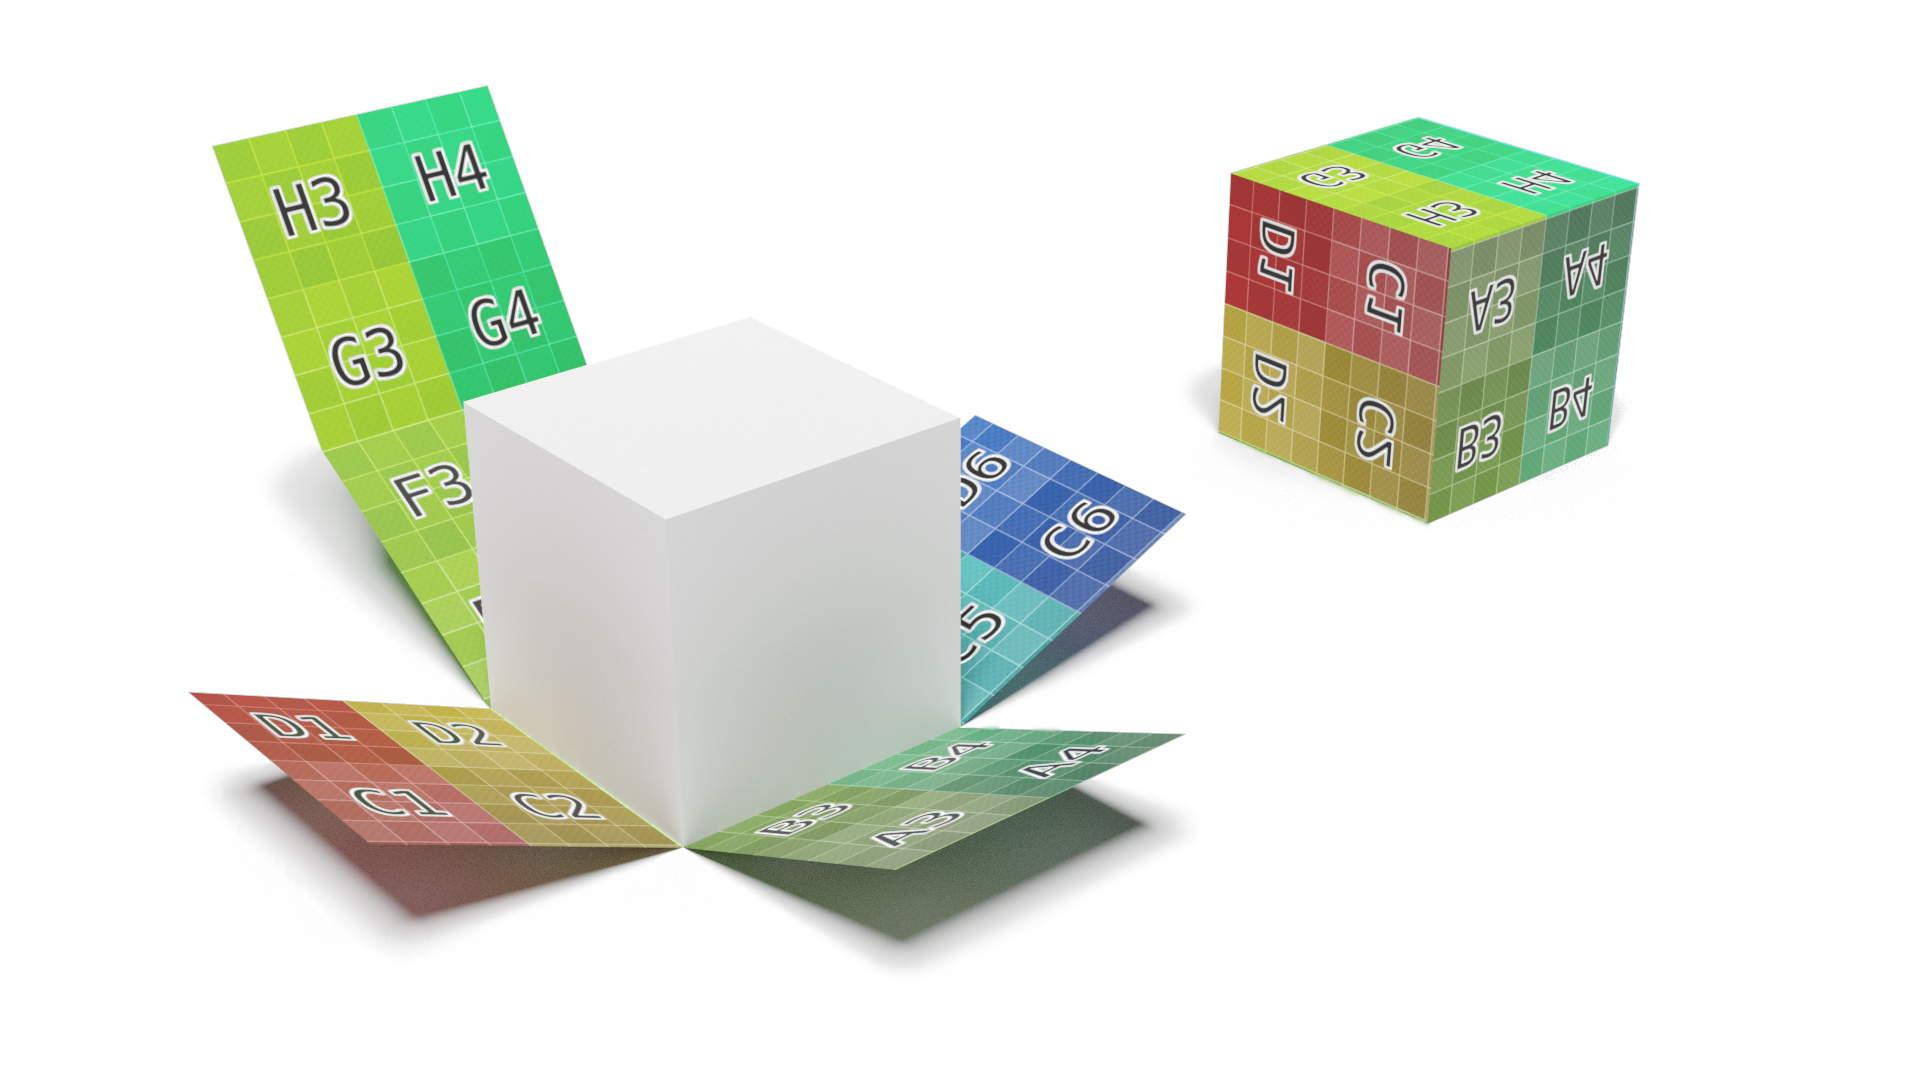
\includegraphics[width=\textwidth]{sections/theory/figures/texture-mapping.png}
    \caption{Texture mapping illustration.}
    \label{fig:texture-mapping}
\end{figure}

\subsection{Ray casting}
Ray casting is the concept of use of ray–surface intersection tests to solve a variety of problems in 3D computer graphics and computational geometry. 
The first use of the term ray casting was made by Scott Roth, in a paper from 1982 titled "Ray casting for modeling solids" \cite{roth-ray-casting}. Raycasting is demonstrated in Figure \ref{fig:raycasting-intersections-example}. A ray is directed towards an object. If it crosses a face, an intersection is registered.

\begin{figure}[h]
    \centering
    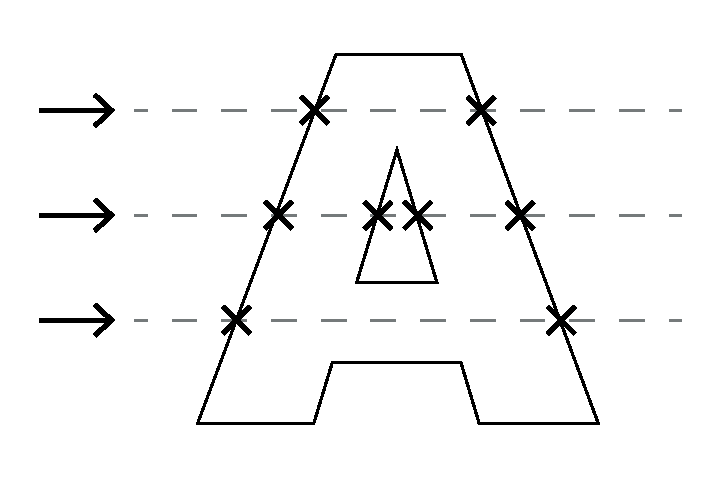
\includegraphics[scale=0.8]{sections/theory/figures/raycast-intersections}
    \caption{Raycasting intersections example.}
    \label{fig:raycasting-intersections-example}
\end{figure}

\subsection{OpenGL}

\subsection{WebGL}
Uses OpenGl ES, a subset of OpenGL. ...

\subsection{three.js}
three.js abstracts away a lot of the manual handling of constructing vertices, faces, setup of WebGL ....

\section{Voxelizer v0.1.3}
Voxelizer v0.1.3 is a JavaScript library for conducting voxelization of 3D models. It features a voxelization algorithm based on raycasting. 

The algorithm used for sampling a model tries to produce a solid voxelization. It samples the front and the back of the model, combines the two results together and tries to fill the in-between gap.

The library is not bundled. Hence, it is not possible to use the program out of the box in a browse. One are limited to Node.js, or setting up a build system involving a module bundler like Webpack or Rollup.

Although, it is very hard to extend, and understand. It is missing documentation...
Voxelizer produces unsatisfactory voxelization results. Several of the voxelizations contains holes.
The software can only produce a solid model. This is because of it's limiting raycasting. It only samples one side of the model. In turn, this results in 
Meaning, it is only able to produce usable results when . When not using the "filled" mode, the voxelizations are

When it comes to the quality of the actual code, it refle

\section{3D Modeling}
Describe the process and fundamentals of 3D modeling.
UV mapping
Procedural generated texture..
Texture baking
Use Blender etc...
